\documentclass[../document.tex]{subfiles}
\begin{document}
\section{Results}
In the section we show and evaluate the models results. We will start by presenting to the reader the networks score on each metric, then we will use the best models to predict the traversability of real world terrain. Finally, we will use handcrafted patches, for example a wall of a certain height in a specific position, to test the robustness of the network by trying to highlighting its behaviour.
\subsubsection{Experiment Setup}
We run all the experiment on a work station with Ubuntu 18.10 operating system. The machine is equipped with a Ryzen 2700x, a powerful CPU with 8 cores and 16 threads, and a NVIDIA 1080 GPU with 8GB of dedicated RAM.
For the classification task, we select a threshold of $0.2m$ on a time window of two seconds to label the patches, meaning that a patch with an advancement less than $20$ centimeters is labeled as \emph{no traversable} and viceversa. We minimise the binary Cross Entropy.
On the other hand, for regression, we did not label the patch and directly regress on the advancement for a given time window while minimising the Mean Square Error (MSE). 
To train the network we follow the best practice on residual network \cite{he2015deep} using Standard Gradient Descent with momentum set to $0.95$ and weight decay to $1e-4$ with an initial learning rate of $1e-3$.
We fix the maximum number of train epochs to $30$ and reduce the learning rage on platuoe \todo{fix this typo} by a factor of $0.1$ with a patience of $4$. We used early stopping to stop the training if the validation accuracy does not increase in $6$ epochs.
\subsubsection{Experimental validation}
We select as \emph{validation} ten percent of the training data. We remain to the reader that we store each run of \emph{Krock} as a \emph{.csv} file. So, to avoid any biases, we used completely different dataframes, meaning that train and validation sets are composed by non overlapping data from the simulations.
\todo[inline]{add more maps if we add them to the test set}
\subsubsection{Metrics}

\paragraph{Classification:} To evaluate the model's classification performance we used two metrics: \emph{accuracy} and \emph{AUC-ROC Curve}. Accuracy scores the number of correct predictions made by the network while AUC-ROC Curve represents degree or measure of separability, informally it tells how much model is capable of distinguishing between classes. For each experiment, we select the model with the higher AUC-ROC Curve during training to be evaluated on the test set.
\paragraph{Regression:} We used the Mean Square Error to evaluate the model's performance.
\subsection{Quantitative Results}
The following table shows the final results on various test dataset made by using real-world heightmaps. 
% \begin{table*}
%     \centering
%     \ra{1.2}
%     \cs{3}
%     \footnotesize
%     \caption{
%     %Description of the heightmaps and the evaluation datasets generated from them.
%     For each dataset we report accuracy (ACC) and the area under the ROC curve (AUC) to compare our approach (CNN) to a Feature Based (FB) and a Baseline (BL) classifier.
%     %
%     %The combined evaluation dataset in real maps is equivalent to traversing \SI{21}{\km} while the synthetic dataset is equivalent to \SI{9}{\km}.
%     %Performance of CNN, feature-based (FB) and baseline approaches. Accuracy (ACC) and area under the ROC curve (AUC) metrics are from a synthetic dataset $D_\text{eval,syn}$  and the real datasets: $D_\text{eval,sullens}$, $D_\text{eval,gravelpit}$ and $D_\text{eval,quarry}$.
%     }
%     \label{tab:fullevaluation}
%     \begin{tabular}{@{}llccccccccccccccccccc@{}}
%     \toprule
%        & & & \multicolumn{10}{c}{Quantitative evaluation in simulation} &&  &&  &&  &&  \\
%          \cmidrule{4-13}
%        \multicolumn{2}{c}{Dataset} & & &  & \multicolumn{2}{c}{CNN} && \multirow{2}{*}{\makecell{Size \\ ( ($\SI{}{m})\times$maps ) }} && \multirow{2}{*}{\makecell{Resolution \\ ($\SI{}{cm/px}$)}} && \multirow{2}{*}{Mapping} \\
%         \cmidrule{1-2}  \cmidrule{6-7} \cmidrule{9-10} \cmidrule{12-13}
%         Type     &  Name  && Samples  &    &  ACC  &  AUC   &&  &&  &&  && \\
%     \toprule
%   \multirow{2}{*}{Synthetic}  & Training   && 450k && - & - && - &  $(10\times10\times2)\times30$ && 2 && -\\
%   %\hdashline
%   %\cdashline{2-21}[0.5pt/5pt]
%                              & Evaluation  && 150k && 0.926 & 0.970 && 0.703 & 0.746 && 0.544 & 0.527 && - && $(10\times10\times2)\times10$ && 2 && - \\
%   \cmidrule{2-21}
%   %\cdashline{2-21}[2.5pt/5pt]
%   \multirow{6}{*}{\makecell[l]{Real\\evaluation}}   & Quarry    && 100k  && 0.819 & 0.840 && 0.723 & 0.762 && 0.542 & 0.499 && - && $32\times32\times10$ && 2 && Fixed-wing \\
%                            & Sullens  && 100k  && 0.858 & 0.884 && 0.781 & 0.799 && 0.527 & 0.501 && - && $30\times30\times10$ && 3 && Fixed-wing  \\
%                            & Gravelpit && 60k  && 0.832 & 0.839 && 0.769 & 0.802 && 0.577 & 0.504 && - && $(10\times20\times4)\times3$ && 5 && Fixed-wing  \\
%                            & ETH-ASL  &&  30k  && 0.887 & 0.921 && 0.789 & 0.817 && 0.492 & 0.511 && - && $7\times7\times1$ && 2 && Quadcopter \\
%                            & Slope    &&  40k  && 0.864 & 0.875 && 0.761 & 0.780 && 0.530 & 0.501 && Yes && $7\times7\times2.5$ && 2 && Handheld \\
%                            & Bars     &&  20k  && 0.961 & 0.980 && 0.829 & 0.863 && 0.493 & 0.498 && Yes && $10\times10\times1$ && 5 && CAD \\
%     \bottomrule
%     \end{tabular}
%     %\bigskip
%     \normalsize
%   \end{table*}
  
%\bigskip
% \normalsize
% \end{table*}


\begin{table*}[h]
    \centering
    \ra{1.2}
    
    \begin{tabular}{@{}llccccc@{}}
    \toprule
    % \multicolumn{8}{c}{Quantitative evaluation in simulation} \\
    \multicolumn{2}{c}{Dataset} && \multicolumn{2}{c}{ResNet} & Size & Resolution(cm/px) \\
    \cmidrule{1-2} \cmidrule{4-5}
    Type     &  Name  & Samples & ACC  &  AUC    & & \\
    \toprule
      \multirow{2}{*}{Synthetic}  & Training   & TODO & - & - & & 2\\
      &  Evaluation   & TODO &   &  & & 2 \\
      \cmidrule{2-7}
    \multirow{3}{*}{\makecell[l]{Real\\evaluation}} & Quarry & TODO & & & & 2\\
    & Quarry & TODO & & & & \\
    & Quarry & TODO & & & & \\

    \bottomrule    %    \multicolumn{2}{c}{Dataset} & & &  & \multicolumn{2}{c}{CNN} && \multirow{2}{*}{\makecell{Size \\ ( ($\SI{}{m})\times$maps ) }} && \multirow{2}{*}{\makecell{Resolution \\ ($\SI{}{cm/px}$)}} && \multirow{2}{*}{Mapping} \\

\end{tabular}
\caption{Todo}

\end{table*}
Moreover, we would like to also show the different steps we made to reach this result. The following table shows the metric's score without any data-augmentation.
Adding dropout increases the results.
\todo[inline]{table with results}
With dropout plus coarse dropout.
\todo[inline]{table with results}
\subsection{Qualitative results}
We qualitative evaluate the models in real world scenarios by computing the traversability probability for each map with different rotation. Specifically, we used a sliding window to extract the patches from the heightmaps and colour by blue the relative region with the corresponding traversability probability. A brighter colour yields an higher probability. For each map we show the traversability from bottom to top, top to bottom, left to right and right to left since those are the most human understandable.
We will start by showing the traversability probability on the \emph{Quarry} assuming \emph{Krock} is walking from bottom to top.
\todo[inline]{add quarry textures from bottom to top}
Thanks its special locomotion, \emph{Krock} can traverse the big slopes in the top part of them map while obliously it is stock by big bumps near the bottom as show in the next figures.
\begin{figure}[H]
\centering
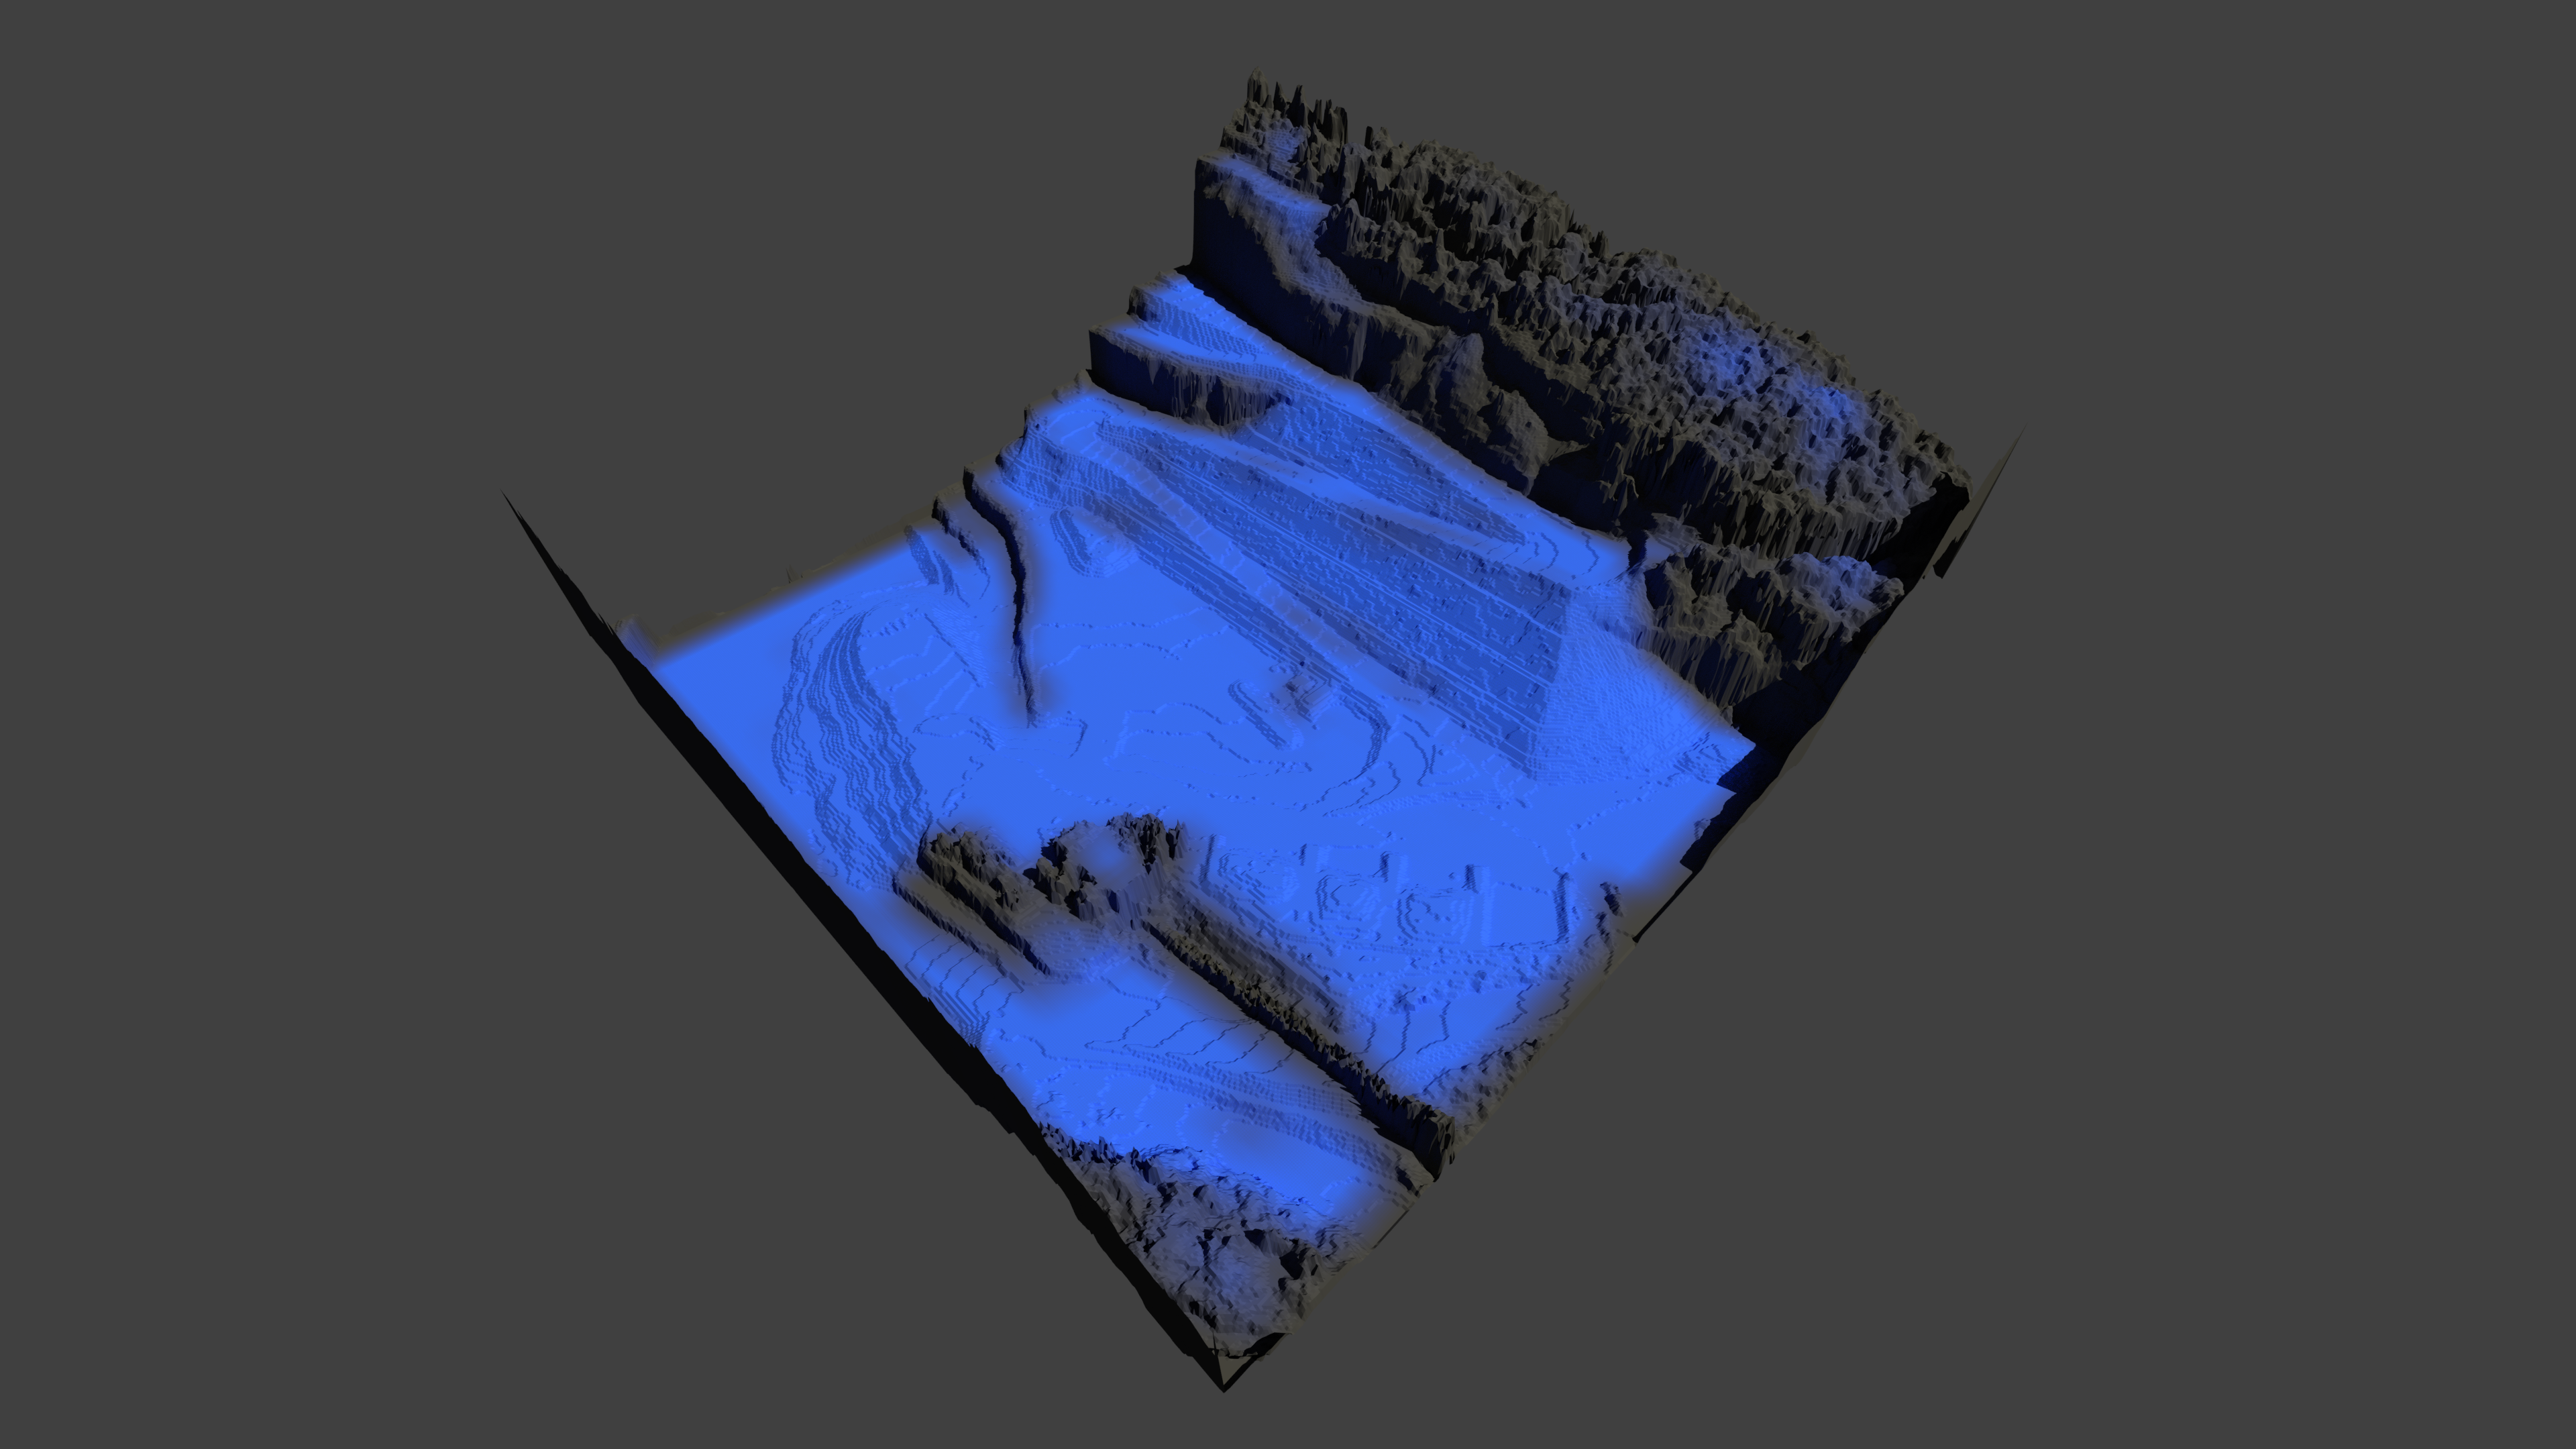
\includegraphics[width=\linewidth]{../img/4/traversability/quarry/querry-big-10-270.png}
\end{figure}
\todo[inline]{add figure of krock traversing the big slopes and getting stop near the bottom}
To convince the reader that those slopes can be traverse, we run \emph{Krock} on them directly from the simulator.
\todo[inline]{image of one extracted patch from quarry and one run on the simulator} 

\end{document}